\documentclass[letterpaper]{article}
\usepackage[submission]{aaai2027}
\usepackage[hyphens]{url}
\usepackage{graphicx}
\urlstyle{rm}
\def\UrlFont{\rm}
\usepackage{natbib}
\usepackage{caption}
\usepackage{subcaption}
\usepackage{amsmath}
\usepackage{algorithm}
\usepackage{algorithmic}
% Render algorithmic comments as a clean right-triangle marker instead of the
% default "// ..." C-style comment, and provide a phase-header helper so that
% section markers inside the pseudocode align consistently.
\renewcommand{\algorithmiccomment}[1]{\hfill$\triangleright$ \textit{#1}}
\newcommand{\PHASE}[1]{\STATE \textit{\underline{#1}}}
\usepackage{booktabs}
\usepackage{multirow}
\usepackage{pifont}
\usepackage{xcolor}
% Listings for verbatim prompt/schema reproduction in the appendix. AAAI-safe:
% no background color, monospace footnotesize, line numbers within the column.
\usepackage{newfloat}
\usepackage{listings}
\DeclareCaptionStyle{ruled}{labelfont=normalfont,labelsep=colon,strut=off}
\lstset{%
  basicstyle={\footnotesize\ttfamily},
  breaklines=true,breakatwhitespace=false,
  columns=fullflexible,keepspaces=true,
  showstringspaces=false,tabsize=2,
  aboveskip=4pt,belowskip=4pt,
  xleftmargin=1em,frame=none}
\floatstyle{ruled}
\newfloat{listing}{tb}{lst}{}
\floatname{listing}{Listing}
% Loosen float placement so full-width table*/figure* floats settle near their
% references instead of being pushed to the end pages.
\setcounter{topnumber}{2}
\setcounter{bottomnumber}{2}
\setcounter{totalnumber}{4}
\renewcommand{\topfraction}{0.92}
\renewcommand{\bottomfraction}{0.7}
\renewcommand{\textfraction}{0.08}
\renewcommand{\floatpagefraction}{0.7}
\renewcommand{\dbltopfraction}{0.92}
\renewcommand{\dblfloatpagefraction}{0.7}
\frenchspacing

\pdfinfo{
/TemplateVersion (2027.1)
}

\setcounter{secnumdepth}{0}

\title{DarwinTrade: Auditable Self-Evolution for Multi-Analyst LLM Portfolio Trading}
\author{
    Anonymous Submission
}
\affiliations{
}

\begin{document}

\maketitle

\begin{abstract}
Large language models (LLMs) can integrate prices, news, fundamentals, and other
financial evidence for portfolio decisions. However, existing LLM trading agents
typically adapt by feeding unstructured reflection back into a single
model-generated action, entangling analyst research, portfolio construction, and
execution; as a result, it is difficult to identify which part of the policy
evolved, whether realized outcomes justify that change, and whether the updated
policy stays within specified risk controls. In this paper, we introduce
DarwinTrade, a self-evolving portfolio framework that decomposes policy adaptation
into auditable feedback loops and keeps LLM-based research separate from a
deterministic allocator and execution. DarwinTrade self-evolves at three timescales.
At the analyst level, an online information-coefficient aggregator evolves the
regime-conditioned influence of four LLM analysts from delayed next-open returns.
At the tactical level, short-lived guards adapt to recent market conditions and
expire automatically. At the strategic level, long-lived policy changes are
restricted to validated allocator parameters and reverted whenever a logged
performance condition is violated. In this way, analyst, tactical, and strategic
self-evolution remain independently auditable, and the LLM never modifies execution
code. With transaction costs on a fixed 20-stock universe, DarwinTrade achieves
returns of $12.1\%$ and $10.9\%$, with Sharpe ratios of $2.07$ and $2.56$, in the
StockBench Rising-Market Window and a later Down-Market Window, respectively.
Disabling all three self-evolution mechanisms reduces Sharpe from $2.07$ to $0.94$
and deepens maximum drawdown from $-6.7\%$ to $-15.2\%$ in the Rising-Market Window,
showing that structured, auditable self-evolution---rather than a single
unstructured adaptation step---drives DarwinTrade's performance.
\end{abstract}

\section{Introduction}

Large language models (LLMs) can synthesize prices, news, fundamentals, and other
financial evidence for portfolio decisions
\citep{zhang2024finagent,liu2025finpos,rashid2026finanalyst}. Yet sequential portfolio
management also requires an explicit account of how market conditions, analyst
relevance, positions, and realized outcomes change subsequent decisions
\citep{liu2025finpos}.

Existing LLM trading systems commonly feed reflections or stored experience into the
next model-generated action
\citep{yu2023finmem,xiao2024tradingagents,tian2025tradinggroup,chen2025threestrader}.
This entangles analyst evaluation, constrained portfolio construction, and policy
adaptation, making it difficult to identify what changed, preserve the temporal order
of decisions and outcomes, and enforce risk controls. Recent audits similarly show
that missing intermediate traces and underspecified execution assumptions hinder
diagnosis and reproducibility
\citep{yao2026execution,qu2026clqt,li2026nextfund}.

\begin{figure}[t]
\centering
\makebox[\columnwidth][c]{%
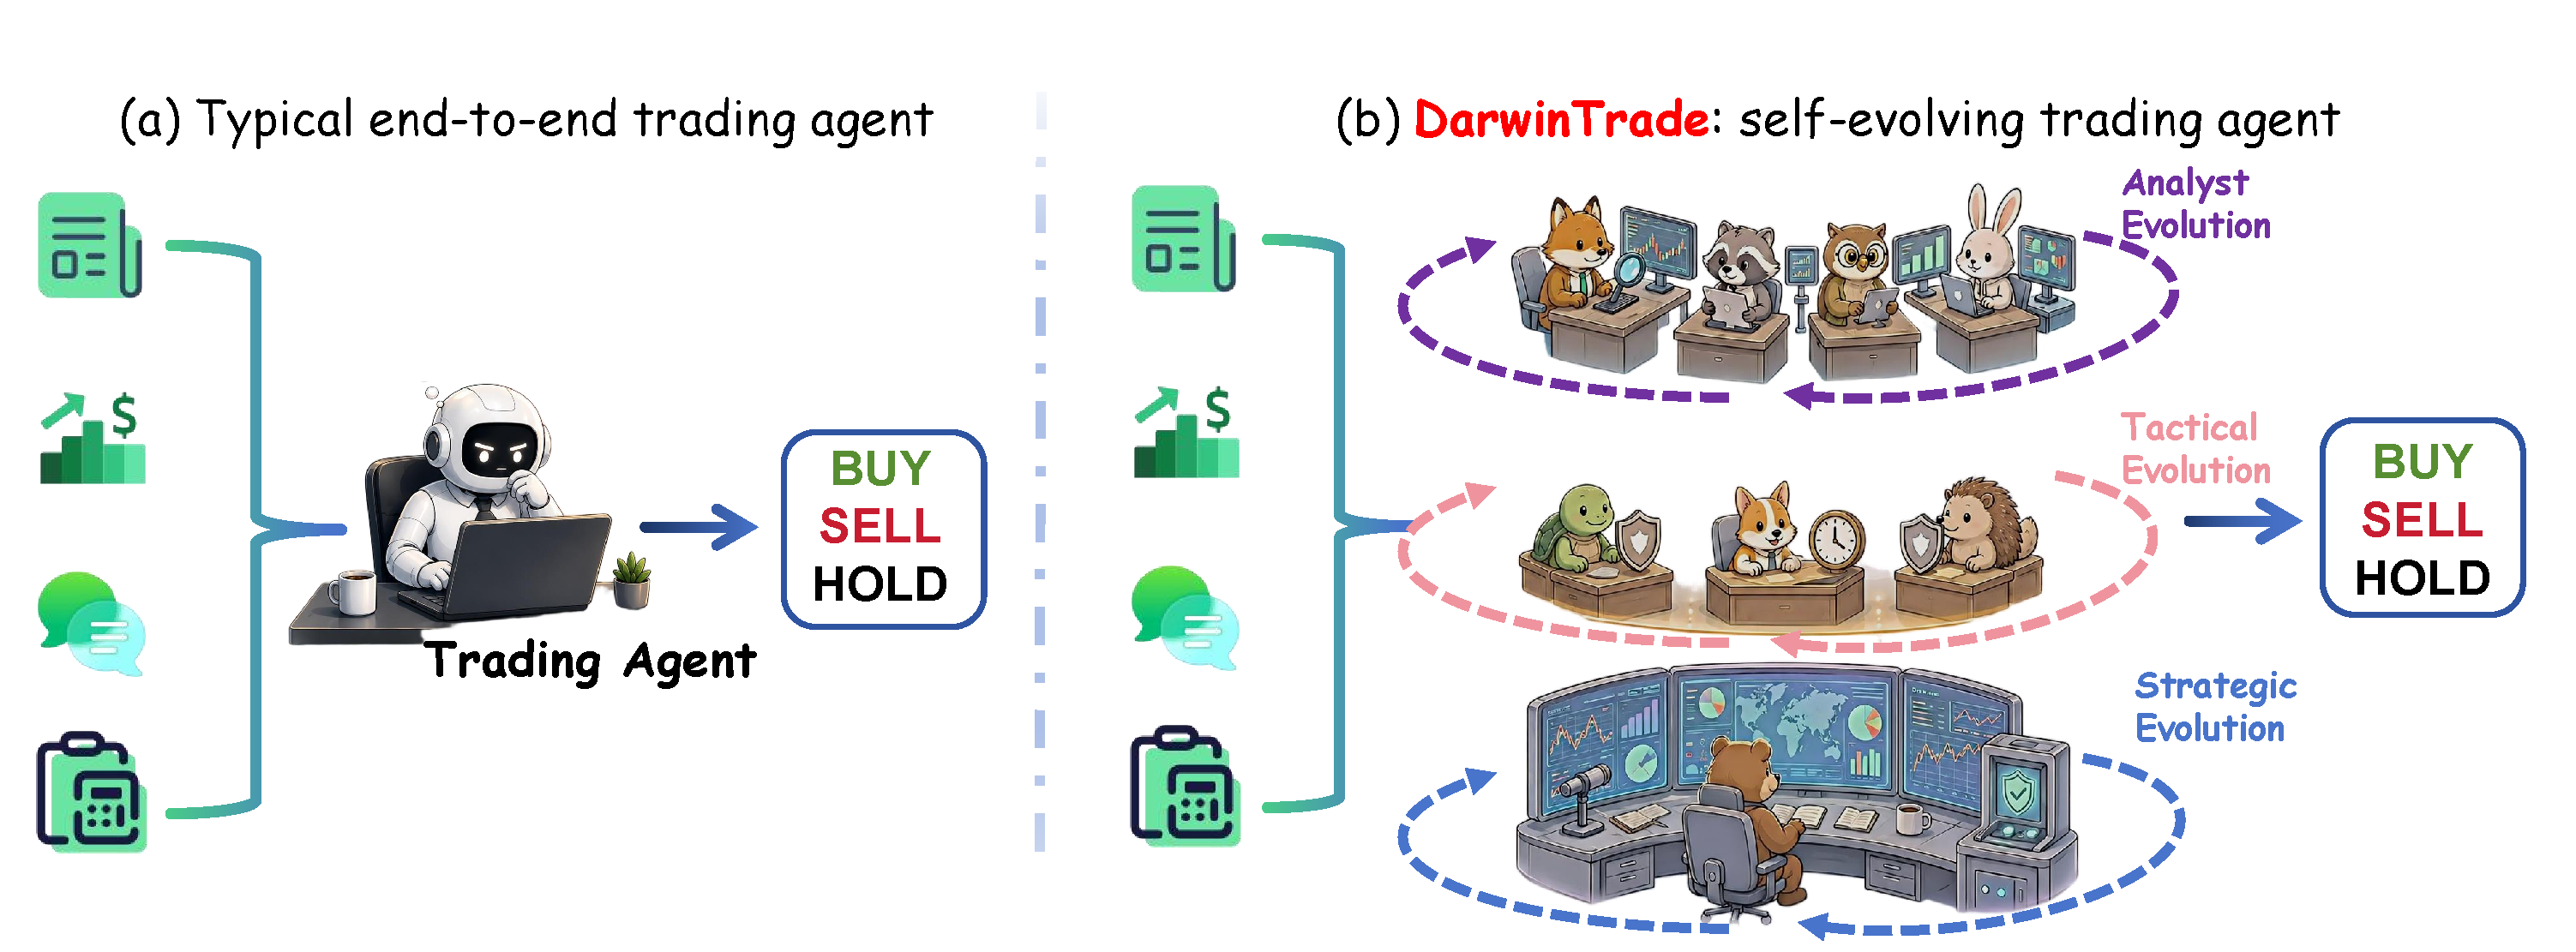
\includegraphics[width=1.08\columnwidth]{Figures/intro_figure.pdf}}
\caption{Comparison between an end-to-end LLM trading agent and DarwinTrade.
\textbf{Left:} one LLM combines research, allocation, and learning. \textbf{Right:}
DarwinTrade self-evolves analyst reliability and portfolio policy from realized
outcomes, while a deterministic allocator controls execution.}
\label{fig:intro}
\end{figure}

To address this problem, we propose DarwinTrade, an auditable self-evolving portfolio
framework that separates research, policy updates, and execution
(Figure~\ref{fig:intro}). Four LLM analysts produce structured asset scores, while an
online information-coefficient (IC) aggregator updates their regime-conditioned
influence from delayed next-open returns. A deterministic allocator then converts the
aggregate signal into constrained long/short weights. DarwinTrade further separates
short-lived tactical guards from long-lived strategic changes: tactical actions expire,
whereas strategic updates are restricted to validated allocator parameters and subject
to automatic rollback. Because outcomes are committed one bar after each decision and
the LLM cannot edit execution code, every update remains attributable to analyst
influence, a temporary risk constraint, or an allocator parameter.

We evaluate DarwinTrade with transaction costs on a fixed 20-stock universe in the
StockBench Rising-Market Window \citep{chen2025stockbench} and a later Down-Market
Window. DarwinTrade returns $12.1\%$ and $10.9\%$, with Sharpe ratios of $2.07$ and
$2.56$, respectively. In the Rising-Market Window, disabling all evolution reduces
Sharpe from $2.07$ to $0.94$ and deepens maximum drawdown from $-6.7\%$ to $-15.2\%$.

Our contributions are threefold: \textbf{(i)} an auditable architecture separating
three evolution layers from deterministic execution; \textbf{(ii)} delayed,
regime-conditioned updates of heterogeneous analyst influence; and \textbf{(iii)}
expiring tactical interventions and validated strategic updates with automatic
rollback.

\section{Related Work}

LLM trading agents commonly combine role specialization, memory, and reflection.
FinMem, FinAgent, TradingAgents, and FinCon revise later decisions from stored
outcomes or role-specific feedback
\citep{yu2023finmem,zhang2024finagent,xiao2024tradingagents,yu2024fincon}, while
QuantAgent, TradingGroup, and 3S-Trader adapt generated programs, styles, or
stock-selection strategies
\citep{wang2024quantagent,tian2025tradinggroup,chen2025threestrader}, and others make
position sizing, downside risk, and specialist evidence more explicit
\citep{liu2025finpos,liu2025finrs,rashid2026finanalyst}. However, they generally do
not maintain analyst reliability, expiring tactical interventions, and validated
allocator changes as three separately logged operative states.

Recent benchmarks and audits emphasize sequential validity and traceability.
StockBench, LiveTradeBench, and AI-Trader show that static capability does not
necessarily transfer to live portfolio performance
\citep{chen2025stockbench,yu2025livetradebench,fan2025aitrader}. Execution audits,
CLQT, NextFund, and TradeLens further expose the importance of point-in-time controls,
intermediate decision traces, and profit--cost attribution
\citep{yao2026execution,qu2026clqt,li2026nextfund,duan2026tradelens}. Related studies
identify look-ahead leakage, passive exposure, and regime-dependent performance as
additional confounds
\citep{glasserman2024lookahead,fu2025newquant,zhu2026ktdfin,jeon2026blindtrade}.
DarwinTrade addresses these concerns through delayed feedback, exposure diagnostics,
separately logged evolution states, and deterministic order generation.

DarwinTrade also connects reflective agents with classical portfolio construction.
ReAct and Reflexion update behavior from environmental feedback
\citep{yao2022react,shinn2023reflexion}, while mean--variance optimization, active
management, and hierarchical risk parity separate forecasts from risk-controlled
allocation \citep{markowitz1952portfolio,grinold2000active,lopezdeprado2016hrp};
DarwinTrade evolves research and portfolio-control states from realized outcomes yet
retains a deterministic allocator. Table~\ref{tab:related} compares these update
layers in
representative LLM trading systems.

\begin{table}[t]
\centering
\small
\setlength{\tabcolsep}{4.5pt}
\renewcommand{\arraystretch}{1.05}
\newcommand{\rh}[1]{\rotatebox{90}{#1\,}}
\begin{tabular}{@{}l cc cc cc@{}}
\toprule
& \multicolumn{2}{c}{Analyst} & \multicolumn{2}{c}{Tactical}
& \multicolumn{2}{c}{Strategic} \\
\cmidrule(lr){2-3}\cmidrule(lr){4-5}\cmidrule(lr){6-7}
System & \rh{Present} & \rh{Evolving} & \rh{Present} & \rh{Evolving}
& \rh{Present} & \rh{Evolving} \\
\midrule
FinMem          & \ding{55} & \ding{55} & \ding{51} & \ding{51} & \ding{55} & \ding{55} \\
FinAgent        & \ding{55} & \ding{55} & \ding{51} & \ding{51} & \ding{55} & \ding{55} \\
TradingAgents   & \ding{51} & \ding{55} & \ding{51} & \ding{51} & \ding{51} & \ding{55} \\
FinCon          & \ding{51} & \ding{51} & \ding{51} & \ding{51} & \ding{55} & \ding{55} \\
QuantAgent      & \ding{51} & \ding{55} & \ding{55} & \ding{55} & \ding{51} & \ding{51} \\
% TradingGroup    & \ding{51} & \ding{55} & \ding{51} & \ding{51} & \ding{51} & \ding{51} \\
\textbf{DarwinTrade} & \ding{51} & \ding{51} & \ding{51} & \ding{51} & \ding{51} & \ding{51} \\
\bottomrule
\end{tabular}
\caption{Functional coverage in representative LLM trading systems.
``Present'' marks whether the layer exists at all (\ding{51}\,yes / \ding{55}\,no);
``Evolving'' marks whether realized feedback updates the layer's operative state.
Analyst evolution changes role influence, tactical evolution changes near-term
decisions, and strategic evolution changes executable portfolio-control state.}
\label{tab:related}
\end{table}


\section{Method}

DarwinTrade is a self-evolving portfolio framework that continually revises its
trading policy from realized outcomes, while keeping LLM-based research separate
from a deterministic allocator and execution. Its design follows one principle:
every policy change must be attributable to a specific signal, a realized outcome,
and a bounded policy component, so that self-evolution can be audited rather than
hidden inside a single model-generated action. As shown in
Figure~\ref{fig:architecture}, a daily control loop maps multi-source evidence to
role-weighted signals, constrained portfolio weights, and orders, while delayed
realized outcomes drive three self-evolution loops operating at the analyst,
tactical, and strategic timescales.

On trading day $t$, four LLM analysts process market, news, fundamental, and social
evidence dated strictly before $t$. Their structured signals are fused using
regime-conditioned reliability, filtered by any active short-lived tactical guards,
and converted into target weights by a deterministic allocator under the current
strategic policy. DarwinTrade freezes these weights before the opening auction,
using the day-$t$ open only as the fill price. At the next opening auction, realized
open-to-open returns are attached to the stored decision trace and may update future
analyst, tactical, and strategic states. We call one completed decision bar with its
next-open outcome an \emph{episode}, the unit on which the strategic review cadence
is counted. This one-bar delay prevents an outcome from changing the decision that
generated it, a point-in-time discipline also emphasized by recent reproducibility
audits and closed-loop benchmarks \citep{yao2026execution,qu2026clqt}.

The remainder of this section details the three self-evolution loops in turn:
analyst reliability learned from cross-sectional forecast quality
(Section~\ref{sec:analyst-evolution}), short-lived tactical guards that adapt to
recent conditions and expire automatically (Section~\ref{sec:tactical-evolution}),
and long-lived strategic policy restricted to validated allocator parameters
(Section~\ref{sec:strategic-evolution}).
Appendix~\ref{app:pseudocode} states the complete per-bar and periodic control loop
as pseudocode, and Appendix~\ref{app:prompts} reproduces every LLM prompt and
output schema used below.

\begin{figure*}[t]
\centering
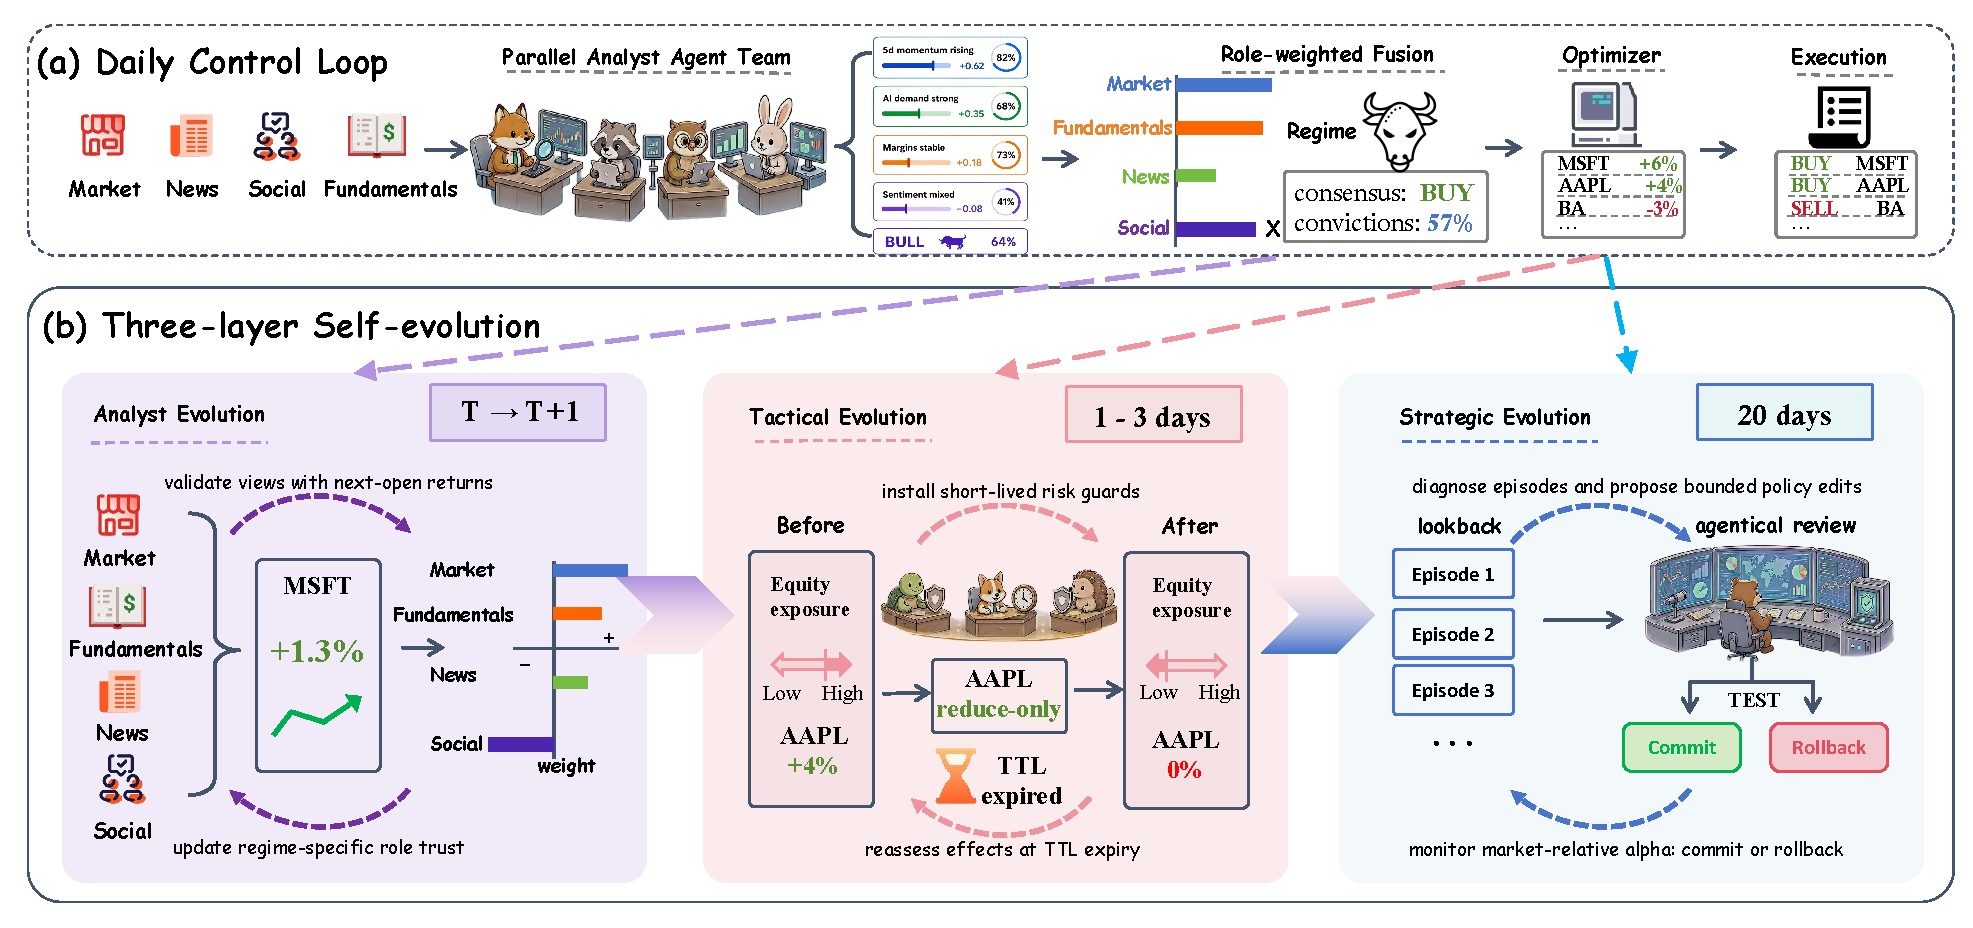
\includegraphics[width=\textwidth]{Figures/method_figure.pdf}
\caption{DarwinTrade architecture. \textbf{Top:} the daily control loop maps
multi-source evidence to role-weighted signals, constrained portfolio weights, and
orders. \textbf{Bottom:} delayed realized outcomes drive self-evolution of analyst
reliability, short-lived tactical guards, and strategic allocator policy.}
\label{fig:architecture}
\end{figure*}

\subsection{Analyst Evolution}
\label{sec:analyst-evolution}

\paragraph{Forward process.}
Because research roles may be reliable under different market conditions---forecast
and trading skill are known to vary materially across regimes
\citep{zhang2025regimefolio,jeon2026blindtrade}---DarwinTrade first identifies the
market regime and then performs regime-conditioned role fusion. The LLM module
$f_{\text{regime}}$ classifies the market as bull, bear, sideways, or volatile
using SPY's $5$- and $20$-bar trailing returns from closes dated before $t$. Here
``volatile'' labels a \emph{trend-disagreement} state in which the short- and
long-horizon trends carry opposite signs, not a high-realized-volatility state,
because such sign disagreement is precisely what erodes trend- and momentum-style
cross-sectional forecasts and thus matters most for analyst gating and long/short
sizing. It returns the regime $\rho_t$ and its confidence under a fixed schema,
falling back to a deterministic trend rule on malformed output. The regime selects
the analyst-evaluation capsules and is not added to the analyst prompts.

For each asset $i$, four role-specific LLM modules process market, news, fundamentals,
and social evidence in parallel. Each analyst $k\in\mathcal{K}$ returns a
directional score $x_{t,i,k}\in[-1,1]$ and confidence $c_{t,i,k}\in[0,1]$ under a
fixed schema, following the role-specialized decomposition of recent financial
agent systems \citep{xiao2024tradingagents,rashid2026finanalyst}; tool traces and
structured outputs are stored in $\tau_t$.
Given the current regime-conditioned role reliability $u_{\rho_t,k,t}$, the fusion
module computes analyst influence $\alpha_{t,i,k}$ and aggregate score $s_{t,i}$ as
\begin{equation}
\alpha_{t,i,k}=u_{\rho_t,k,t}c_{t,i,k},
\qquad
s_{t,i}=\frac{\sum_{k\in\mathcal{K}}\alpha_{t,i,k}x_{t,i,k}}
                  {\sum_{k\in\mathcal{K}}\alpha_{t,i,k}}.
\label{eq:analyst-fusion}
\end{equation}
In Eq.~\ref{eq:analyst-fusion}, reliability $u_{\rho_t,k,t}$ and confidence
$c_{t,i,k}$ enter the fusion weight $\alpha_{t,i,k}$ linearly, whereas cross-role
agreement enters through the normalized signed average $s_{t,i}$, in which roles
voting against the majority sign partially cancel. Position conviction re-weights each
role by the same $\alpha_{t,i,k}$, so confidence enters sizing as $c^2$; we take this
$c^2$ form as the canonical default and contrast it with a linear-$c$ variant in
Appendix~\ref{app:design}. Scores above $0.15$ produce buy
candidates, scores below $-0.15$ produce sell candidates, and intermediate scores
are held out. These fixed thresholds are unchanged across all self-evolution
ablations. The four analyst role prompts and their shared output schema are given
in Appendix~\ref{app:analyst-prompts}.

\paragraph{Self-evolution loop.}
To evolve analyst reliability from realized outcomes, DarwinTrade maintains one
evaluation capsule for each regime--role pair $(\rho,k)$. Each capsule
stores the latest $200$ tuples $(x_{t,i,k},c_{t,i,k},y_{t+1,i},t)$. After removing
the cross-sectional mean of each trade date from both scores and returns,
DarwinTrade computes their Pearson correlation
$\mathrm{IC}_{\rho,k,t}$, following the use of information coefficients to evaluate
cross-sectional forecast quality in active management \citep{grinold2000active}. Let
$n_{\rho,k,t}$ denote the number of observations in
the capsule. The role skill used on the next bar is
\begin{equation}
u_{\rho,k,t}
  =
  \begin{cases}
  u_0, & n_{\rho,k,t}<20,\\
  \max(0,\mathrm{IC}_{\rho,k,t})
    \dfrac{n_{\rho,k,t}}{n_{\rho,k,t}+20}, & n_{\rho,k,t}\geq20.
  \end{cases}
\label{eq:analyst-skill}
\end{equation}
Negative IC therefore removes a warm role instead of reversing its signal, and
shrinkage limits the influence of estimates supported by few observations. If all
warm roles have zero skill, the cold-start value $u_0=0.01$ keeps the system active
while new evidence accrues. Because $y_{t+1,i}$ is unavailable at decision time $t$,
a day-$t$ prediction can change $u_{\rho,k}$ only from day $t+1$ onward, which then
updates the role weights in Eq.~\ref{eq:analyst-fusion}---a strictly delayed
analyst-evolution loop.

\subsection{Tactical Evolution}
\label{sec:tactical-evolution}

\paragraph{Forward process.}
Short-lived events may require immediate risk control that should not permanently
change the allocation policy, much as position-aware agents separate directional
reasoning from exposure adjustment \citep{liu2025finpos,liu2025finrs}. DarwinTrade
therefore maintains a tactical state $\mathcal{U}^T_t$ with an avoid set, a
reduce-only set, a portfolio haircut, and a time-to-live: avoided symbols cannot open
new positions, reduce-only symbols cannot increase absolute exposure, and the haircut
scales target sizes in $[0.4,1.0]$. Every guard expires after one to three trading
days, so a tactical response constrains the next decision without silently becoming
permanent policy.

\paragraph{Self-evolution loop.}
After the next-open portfolio return $y^{\mathrm{pf}}_t$ of the preceding episode
becomes available, a reflection module summarizes the dominant one-day failure as
$q^T_t=f_{\text{tac-reflect}}(\tau_{t-1},y^{\mathrm{pf}}_t,\mathcal{U}^T_t)$, and an
evolution module turns this into a guard action that the state then absorbs:
\begin{equation}
\eta^T_t = f_{\text{tac-evolve}}\!\left(q^T_t, \mathcal{U}^T_t\right),
\qquad
\mathcal{U}^T_{t+1} = \operatorname{Install}\!\left(\mathcal{U}^T_t, \eta^T_t\right).
\label{eq:tactical-loop}
\end{equation}
The action $\eta^T_t$ may install an avoid, reduce-only, or haircut guard, but an
empty action is also valid. Each installation logs its anchor NAV and post-install
return at expiry, so $f_{\text{tac-evolve}}$ can avoid repeating interventions that
previously harmed performance. The tactical reflection and evolution prompts and the
guard schema appear in Appendix~\ref{app:control-prompts}.

\subsection{Strategic Evolution}
\label{sec:strategic-evolution}

\paragraph{Forward process.}
While the tactical state handles short-lived risks, persistent allocation problems
require changing the long-lived policy, as also explored through outcome-driven
strategy or style revision in reflective trading agents
\citep{tian2025tradinggroup,chen2025threestrader}. DarwinTrade parameterizes
the deterministic allocator by the strategic policy $\boldsymbol{\pi}_t$. Given
the guarded signals $\widetilde{\mathcal{S}}_t$, current portfolio $P_t$, and
historical returns $\mathcal{R}_{<t}$, the allocator produces
\begin{equation}
\begin{aligned}
\boldsymbol{w}_t&=\operatorname{Allocate}\!\left(
    \widetilde{\mathcal{S}}_t,P_t,\mathcal{R}_{<t};\boldsymbol{\pi}_t\right),\\
&\text{s.t. } |w_{t,i}|\leq w_{\max,t},\ \ \textstyle\sum_i|w_{t,i}|\leq G_t.
\end{aligned}
\label{eq:strategic-allocation}
\end{equation}
where $G_t$ is the gross-exposure budget (default $0.95$) and $w_{\max,t}$ the
per-name cap. Gross exposure is split between long and short legs by the confidence
mass on each side. The policy selects one of nine allocator modes spanning classical
mean--variance, active-allocation, and hierarchical-risk-parity families
\citep{markowitz1952portfolio,grinold2000active,lopezdeprado2016hrp}; covariance-based
modes require at least $20$ per-asset returns and otherwise revert to confidence
weighting (Appendix~\ref{app:allocator}). The allocator holds no directional prior,
so net exposure is set by the cross-sectional signal distribution.

\paragraph{Self-evolution loop.}
A single episode provides insufficient evidence for changing a long-lived policy.
Recent live and repeated-run studies likewise show that short samples can reverse
agent rankings or leave module effects within run-to-run noise
\citep{rashid2026finanalyst,qu2026clqt}.
Therefore, after every three completed episodes, DarwinTrade forms a twenty-day
history $\mathcal{H}^S_j$ for review cycle $j$. A review module diagnoses this
history as $z^S_j=f_{\text{str-review}}(\mathcal{H}^S_j,\boldsymbol{\pi}_j)$, and a
policy-author module proposes a restricted change together with its evaluation
horizon $H_j$, loss threshold $\varepsilon_j$, and reference mode $m_j$:
\begin{equation}
(\Delta\boldsymbol{\pi}_j,H_j,\varepsilon_j,m_j)
  = f_{\text{str-policy}}\!\left(z^S_j,\boldsymbol{\pi}_j,\Omega\right),
\label{eq:strategic-evolution}
\end{equation}
where $\Omega$ is the allowed parameter set. The candidate
$\boldsymbol{\pi}_j+\Delta\boldsymbol{\pi}_j$ is accepted only after validation
against $\Omega$.
A review can change only the preferred optimizer,
$G\in[0.3,1.0]$, $w_{\max}\in[0.05,1.0]$, the minimum confidence threshold in
$[0,0.6]$, the position-size multiplier in $[0.5,3.0]$, the long/short net-exposure
target $\beta^{\star}\in[-1,1]$, and the drawdown-guard and rebound-entry thresholds
in $[0,1]$. Any unsupported field or out-of-range value is rejected before it
reaches Eq.~\ref{eq:strategic-allocation}.

To prevent an ineffective change from persisting, each accepted proposal carries an
evaluation horizon $H_j\in[1,30]$, a loss threshold
$\varepsilon_j\in[0.005,0.15]$, and a reference mode $m_j$. Letting
$g_{m_j}(t_j,t)$ be the monitored performance from installation bar $t_j$ through
bar $t$, the system restores $\boldsymbol{\pi}_j$ at the first bar with
$g_{m_j}(t_j,t)<-\varepsilon_j$. The default reference is cumulative
market-relative alpha, $g_{m_j}(t_j,t)=\sum_{\tau=t_j+1}^{t}
(y^{\mathrm{pf}}_{\tau}-y^{\mathrm{mkt}}_{\tau})$, with
$y^{\mathrm{mkt}}_{\tau}$ the equal-weight open-to-open return of the held universe.
If no breach occurs by $t_j+H_j$, the proposal is committed and its outcome enters
$\mathcal{Z}^S_{j+1}$; otherwise the previous policy is restored. Only one proposal
is evaluated at a time. Strategic evolution thus changes only validated allocator
parameters through a logged commit-or-rollback loop and cannot edit the execution
engine. Appendix~\ref{app:control-prompts} lists the strategic prompts, the allowed
set $\Omega$, and the rollback-trigger schema.

\section{Experiments}


\begin{table*}[t]
\centering
\footnotesize
\setlength{\tabcolsep}{3pt}
\begin{tabular}{@{}l l *{5}{r} c *{5}{r}@{}}
\toprule
& & \multicolumn{5}{c}{Rising-Market Window} & & \multicolumn{5}{c}{Down-Market Window} \\
\cmidrule(lr){3-7}\cmidrule(lr){9-13}
Category & Method & Return & \shortstack[r]{Max\\drawdown} & Sharpe & Sortino & \shortstack[r]{Information\\ratio} & & Return & \shortstack[r]{Max\\drawdown} & Sharpe & Sortino & \shortstack[r]{Information\\ratio} \\
\midrule
\multirow{5}{*}{Rule}
 & Buy-and-hold     & $0.008$  & $-0.152$ & $0.25$  & $0.33$  & $-0.29$ & & $-0.044$ & $-0.096$ & $-1.06$ & $-1.60$ & $0.01$ \\
 & Bollinger bands  & $0.034$  & $-0.054$ & $0.73$  & $1.35$  & $-0.37$ & & $-0.013$ & $-0.028$ & $-1.21$ & $-1.90$ & $0.75$ \\
 & ATR bands        & $0.007$  & $-0.067$ & $0.23$  & $0.21$  & $-0.65$ & & $0.007$  & $-0.005$ & $1.54$  & $1.42$  & $1.21$ \\
 & SMA crossover    & $-0.010$ & $-0.124$ & $-0.07$ & $-0.07$ & $-1.19$ & & $0.058$  & $-0.029$ & $1.75$  & $3.39$  & $1.80$ \\
 & WMA crossover    & $-0.065$ & $-0.172$ & $-0.86$ & $-0.81$ & $-1.94$ & & $0.066$  & $-0.025$ & $2.03$  & $3.75$  & $1.86$ \\
\cmidrule(lr){1-13}
\multirow{2}{*}{\shortstack[l]{Machine\\learning}}
 & ARIMA            & $-0.036$ & $-0.113$ & $-0.45$ & $-0.58$ & $-1.23$ & & $-0.052$ & $-0.075$ & $-1.60$ & $-2.13$ & $-0.17$ \\
 & XGBoost          & $-0.044$ & $-0.074$ & $-1.42$ & $-1.46$ & $-1.27$ & & $-0.039$ & $-0.057$ & $-1.92$ & $-2.87$ & $0.14$ \\
\cmidrule(lr){1-13}
\multirow{4}{*}{\shortstack[l]{Classical\\quant}}
 & MVQ + equal-weight  & $-0.052$ & $-0.083$ & $-1.38$ & $-1.79$ & $-1.20$ & & $0.039$ & $-0.058$ & $1.35$ & $1.86$ & $1.72$ \\
 & MVQ + HRP           & $-0.059$ & $-0.092$ & $-1.50$ & $-1.97$ & $-1.21$ & & $0.047$ & $-0.047$ & $1.75$ & $2.72$ & $1.83$ \\
 & MVQ + min-variance  & $-0.063$ & $-0.091$ & $-1.62$ & $-2.13$ & $-1.27$ & & $0.077$ & $-0.039$ & $2.76$ & $4.71$ & $2.39$ \\
 & MVQ + max-Sharpe    & $-0.047$ & $-0.090$ & $-0.99$ & $-1.14$ & $-1.07$ & & $0.026$ & $-0.047$ & $0.90$ & $1.43$ & $1.62$ \\
\cmidrule(lr){1-13}
\multirow{2}{*}{\shortstack[l]{LLM\\agent}}
 & TradingAgents & $-0.000$ & $-0.048$ & $0.05$  & $0.07$  & $-0.72$ & & $-0.020$ & $-0.038$ & $-1.06$ & $-1.92$ & $0.56$ \\
 & FinAgent     & $-0.024$ & $-0.065$ & $-0.66$ & $-0.77$ & $-1.16$ & & $-0.013$ & $-0.046$ & $-0.57$ & $-0.92$ & $0.74$ \\
\midrule
Ours & DarwinTrade & $\mathbf{0.121}$ & $-0.067$ & $\mathbf{2.07}$ & $\mathbf{3.20}$ & $\mathbf{0.18}$ & & $\mathbf{0.109}$ & $-0.039$ & $\mathbf{2.56}$ & $\mathbf{4.24}$ & $\mathbf{2.94}$ \\
\bottomrule
\end{tabular}
\caption{Results in the StockBench Rising-Market Window and the later Down-Market
Window. All methods use the same 20-stock universe and transaction-cost model.
\emph{MVQ} denotes a non-LLM cross-sectional momentum--value--quality composite fed
into the same deterministic allocator DarwinTrade uses, under four portfolio
constructions. Return is cumulative; Sharpe, Sortino, and information ratio are
annualized. Bold marks the best value in each window.}
\label{tab:baselines}
\end{table*}

\subsection{Experimental Setup}

\paragraph{Evaluation Windows and Trading Protocol}
We use a fixed daily U.S. equity universe of 20 large-cap stocks: GS, MSFT, HD, V,
SHW, CAT, MCD, UNH, AXP, AMGN, TRV, CRM, JPM, IBM, HON, BA, AMZN, AAPL, PG, and JNJ.
This liquid, continuously listed basket remains unchanged across both windows and
is not reselected using period-specific information. Each evaluation starts with USD
100,000 and assumes full fills, a 1 bp commission, and 2 bps slippage. Relative
metrics use SPY as the benchmark where available. Full backtest configuration,
the LLM backbone and decoding settings, and baseline hyperparameters are reported
in Appendix~\ref{app:impl}.

The primary evaluation follows the Rising-Market Window distributed with StockBench
\citep{chen2025stockbench}, spanning 2025-03-03 to 2025-06-30. The chronologically
later Down-Market Window spans 2025-12-01 to 2026-03-31, during which SPY falls
$-4.6\%$. The latter changes the market environment while keeping the universe,
controller code, policy space, execution assumptions, and transaction-cost model
fixed. It therefore serves as a regime-shift stress test rather than a separately
tuned setting.

The two windows are evaluated independently. All three evolution states start empty
and adapt only from feedback observed within that window. Thus, ``the same
controller'' refers to frozen code and policy bounds whose evolution restarts for
each evaluation, rather than state transferred from the Rising-Market Window. Each
window contains 83 decision bars and 82 return intervals.


\paragraph{Data Controls}
Research evidence, including price bars, news, fundamentals, and social data, is
admitted only when dated ${<}t$, and prices are adjusted for splits and dividends.
Analyst reliability is learned only from realized post-decision returns, while
allocation remains in the deterministic controller. These controls follow recent
recommendations to make point-in-time admission, execution timing, and intermediate
decision traces explicit \citep{yao2026execution,qu2026clqt,li2026nextfund}.

\paragraph{Baselines}
In the Rising-Market Window, we evaluate the complete $2^3$ factorial over analyst,
tactical, and strategic evolution. The analyst ablation disables online IC updates,
whereas the no-evolution variant disables all three feedback loops. The Down-Market
Window extends the evaluation to a later market environment. We compare against
buy-and-hold, moving-average crossover,
Bollinger bands, ATR bands, ARIMA \citep{box2015time}, XGBoost
\citep{chen2016xgboost}, TradingAgents
\citep{xiao2024tradingagents}, and FinAgent
\citep{zhang2024finagent}. All methods use the same universe, evaluation windows,
and transaction-cost model. 

\paragraph{Metrics and Statistical Tests}
We report cumulative return, maximum drawdown, annualized Sharpe ratio, annualized
Sortino ratio, annualized information ratio against SPY, and trade count. To compare
paired daily returns while accounting for serial dependence, we use a moving-block
bootstrap \citep{kuensch1989jackknife} with block length $5$ and $5000$ resamples,
reporting the paired excess-return estimate
$\Delta_{\Sigma}=100\sum_t(r^{\mathrm{ours}}_t-r^{\mathrm{comp}}_t)$ in percentage
points and $P_+$, the bootstrap probability that $\Delta_{\Sigma}$ is positive.

\subsection{Main Results}

To evaluate whether DarwinTrade remains effective across market regimes, we compare
it with rule-based, machine-learning, and LLM-agent baselines in the Rising-Market
and Down-Market Windows under the common 20-stock universe and transaction-cost
model; Table~\ref{tab:baselines} reports return and risk-adjusted performance, and
Figure~\ref{fig:equity} shows the NAV trajectories.


\paragraph{Comparison with Baselines}
DarwinTrade performs consistently across regimes ($12.1\%$/$2.07$ Sharpe rising,
$10.9\%$/$2.56$ down), whereas the strongest fixed baselines flip with the window:
Bollinger bands lead the rising window ($3.4\%$) but lose $1.3\%$ in the down window,
while WMA shows the reverse ($-6.5\%$ then $+6.6\%$). DarwinTrade thus beats the best
per-window baseline return by $8.7$ and $4.3$ percentage points. With controller
code, policy bounds, universe, and costs fixed, this pattern is consistent with
adaptation inside the specified policy space rather than a different strategy per
window. Feeding a non-LLM momentum--value--quality composite into the \emph{same}
allocator (the four MVQ rows) isolates the analyst layer: every construction loses in
the rising window ($-4.7\%$ to $-6.3\%$) and only modestly profits in the down window
(best: min-variance, $7.7\%$/Sharpe $2.76$), so the shared allocator alone does not
explain DarwinTrade's cross-window gains.

\paragraph{Comparison with External LLM Agents}
DarwinTrade also outperforms TradingAgents ($-0.0\%$/$-2.0\%$) and FinAgent
($-2.4\%$/$-1.3\%$) in both windows. The distinction is not the number of agents:
end-to-end reflection rewrites subsequent model-generated behavior, whereas
DarwinTrade records analyst reliability, temporary risk state, and validated
allocator state separately before deterministic execution, so no reflection can
rewrite order logic---matching evidence that reasoning strength does not
automatically yield stable sequential portfolio performance
\citep{chen2025stockbench,yu2025livetradebench}.

\begin{figure}[t]
\centering
\begin{subfigure}[t]{0.48\columnwidth}
\centering
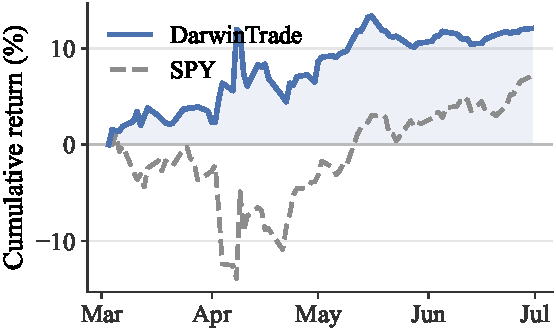
\includegraphics[width=\linewidth]{Figures/darwintrade_window1_equity}
\caption{Rising-Market Window.}
\label{fig:equity-rising}
\end{subfigure}
\hfill
\begin{subfigure}[t]{0.48\columnwidth}
\centering
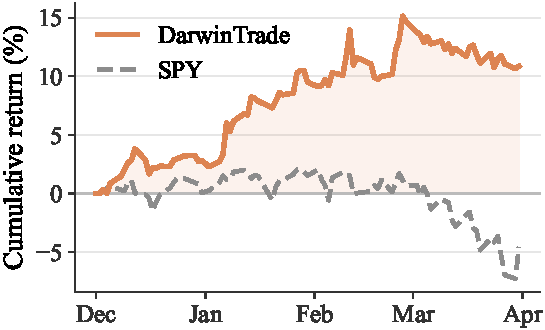
\includegraphics[width=\linewidth]{Figures/darwintrade_window2_equity}
\caption{Down-Market Window.}
\label{fig:equity-down}
\end{subfigure}
\caption{NAV curves of DarwinTrade and SPY in the two evaluation windows.}
\label{fig:equity}
\end{figure}

\section{Analyses}

\subsection{Effects of Three-Layer Self-Evolution}

To separate each evolution layer's contribution from cross-layer coordination, we
run the complete $2^3$ factorial in the Rising-Market Window and inspect
regime-conditioned analyst selection alongside logged tactical and strategic
interventions (Figure~\ref{fig:evolution}, Table~\ref{tab:darwin}).
Table~\ref{tab:darwin} reports four ablation contrasts; the full eight-cell
factorial is in Appendix~\ref{app:factorial}.

\begin{figure}[t]
\centering
\begin{subfigure}[t]{0.46\columnwidth}
\centering
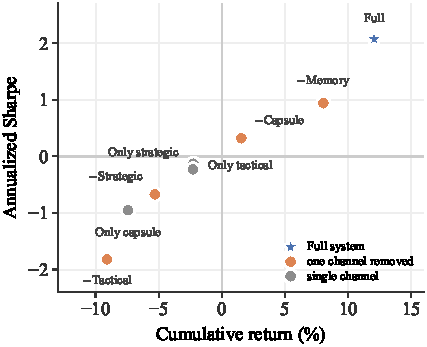
\includegraphics[width=\linewidth]{Figures/fig_factorial_scatter}
\caption{Factorial variants in return--Sharpe space.}
\label{fig:evolution-factorial}
\end{subfigure}
\hfill
\begin{subfigure}[t]{0.46\columnwidth}
\centering
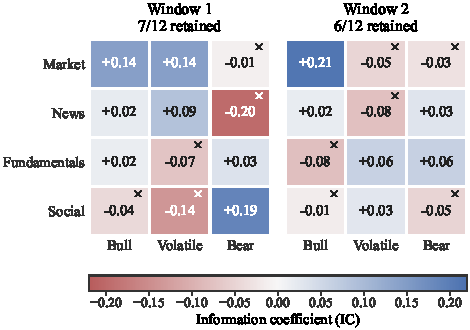
\includegraphics[width=\linewidth]{Figures/fig_capsule_selectivity}
\caption{Regime-conditioned analyst selectivity.}
\label{fig:evolution-analyst}
\end{subfigure}
\caption{Evidence for three-layer self-evolution. (a) Rising-Market Window
factorial variants. (b) Analyst IC by regime; $\times$ marks a non-positive capsule
removed by the aggregation gate.}
\label{fig:evolution}
\end{figure}

The factorial results assign different functions to the three timescales. Removing
tactical evolution causes the largest single-layer loss ($-9.1\%$ return, $-1.82$
Sharpe), consistent with the one-to-three-bar guard being the only loop that can
immediately reduce a newly harmful exposure. Without strategic evolution, return
falls to $-5.3\%$ and maximum drawdown reaches $-16.3\%$, as short-lived guards
cannot replace a persistent change to optimizer or portfolio size. Removing analyst
evolution leaves portfolio controls intact but weakens cross-sectional selection
($1.5\%$ return, $0.32$ Sharpe). These are ablation-level associations, not additive
causal effects: every single-layer-only variant has negative Sharpe, so the layers
must operate on one another's evolving inputs \citep{liu2025finpos,liu2025finrs}.

The static policy still profits, but evolution mainly improves the path of returns:
disabling all three loops yields $8.0\%$ yet halves Sharpe from $2.07$ to $0.94$ and
deepens maximum drawdown from $-6.7\%$ to $-15.2\%$, supporting improved
risk-adjusted adaptation rather than standalone return per update.

Figure~\ref{fig:evolution-analyst} shows why analyst evolution is more than generic
multi-agent averaging. The positive-IC gate suppresses $5$ of $12$ warm capsules in
the Rising-Market Window and $6$ of $12$ in the Down-Market Window; retained
capsules have mean ICs of $0.09$ and $0.07$, versus $-0.09$ and $-0.05$ for removed
ones. Selection is role- and regime-specific---the news analyst, for instance, is
removed on bear-labeled days in the rising window but kept in bull and volatile
regimes---so a role is reused where its delayed evidence stays predictive without
gaining permanent influence \citep{zhang2025regimefolio,jeon2026blindtrade}. This
gating relies on the regime labels: scored against the deterministic trend rule it
follows, the classifier reaches $0.86$ directional agreement in both windows with
errors confined to the adjacent \emph{volatile} state and essentially no bull/bear
sign flips (Appendix~\ref{app:regime}).

\begin{figure*}[t]
\centering
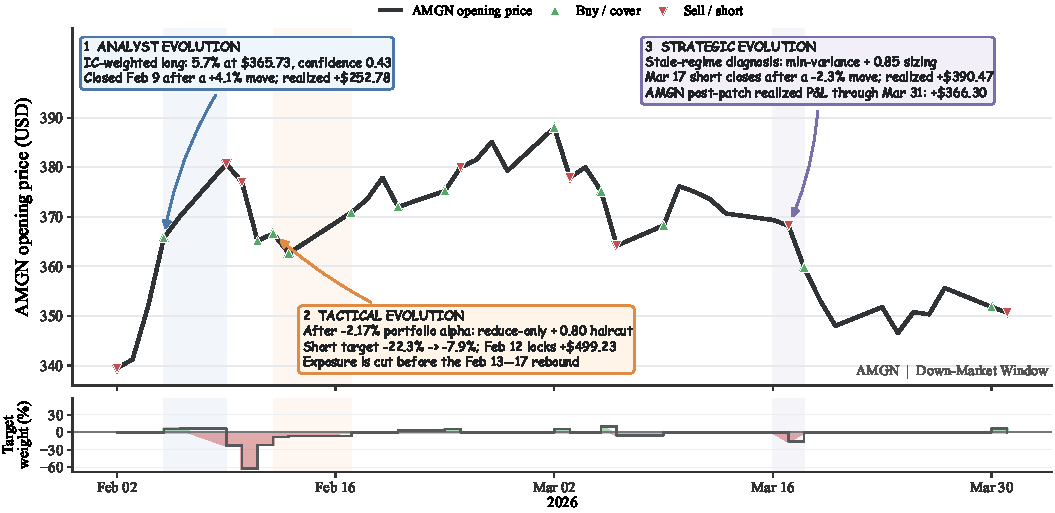
\includegraphics[width=\textwidth]{Figures/fig_case_study_amgn}
\caption{Auditable AMGN case study in the Down-Market Window. The upper panel shows
point-in-time opening prices and executions (up: buy/cover; down: sell/short); the
lower panel shows the deterministic target weight. Numbered callouts mark the analyst
entry (1), the two-bar tactical guard (2), and the strategic allocator update (3),
reporting only fields and outcomes recovered from the run logs.}
\label{fig:case-study}
\end{figure*}

The other layers leave different traces. Tactical interventions expire within one to
three days, limiting a local error without permanently suppressing a symbol, while
strategic evolution edits approved allocator fields and logs the diagnosis, horizon,
and rollback threshold, so its moves toward HRP and risk parity remain bounded and
reversible.

\begin{table}[t]
\centering
\footnotesize
\setlength{\tabcolsep}{5pt}
\begin{tabular}{@{}l r r r@{}}
\toprule
Variant & Return & \shortstack[r]{Max\\drawdown} & Sharpe \\
\midrule
Full            & $\mathbf{0.121}$ & $\mathbf{-0.067}$ & $\mathbf{2.07}$ \\
$-$Tactical     & $-0.091$ & $-0.148$ & $-1.82$ \\
$-$Strategic    & $-0.053$ & $-0.163$ & $-0.67$ \\
$-$Analyst      & $\phantom{-}0.015$ & $-0.112$ & $\phantom{-}0.32$ \\
$-$All evolution & $\phantom{-}0.080$ & $-0.152$ & $\phantom{-}0.94$ \\
\bottomrule
\end{tabular}
\caption{Evolution-layer ablations in the Rising-Market Window.
$-$All evolution disables analyst,
tactical, and strategic feedback loops.}
\label{tab:darwin}
\end{table}

\subsection{Case Study: Auditable Evolution on Amgen}

Because DarwinTrade's central claim is that self-evolution is auditable rather than
hidden, we trace one symbol to show that each timescale acts independently and leaves
an inspectable record. We follow Amgen (AMGN) through the Down-Market Window
(Figure~\ref{fig:case-study}), an auditing example rather than a performance test,
with the full log excerpt in Appendix~\ref{app:case}. Three events act on distinct
timescales. At the analyst timescale, IC-weighted fusion opens a $5.7\%$ long at
$0.43$ confidence and closes it four bars later for $+\$252.78$. When a $-2.17\%$
portfolio-alpha day triggers the tactical timescale, AMGN is placed on a two-bar
reduce-only list with a $0.80$ haircut, which trims a profitable short from $-22.3\%$
to $-7.9\%$, removes exposure before the February 13--17 rebound, and then expires
automatically. At the strategic timescale, a stale-regime diagnosis edits only
approved allocator fields---switching the optimizer to minimum-variance with a $0.85$
size multiplier and logging the horizon and rollback threshold---so the March 17
short is sized down and the symbol accumulates $+\$3.07$k. Each event is attributable
to a specific trigger, outcome, and bounded policy component, inspectable on its own
rather than as one post-hoc reflection.

\subsection{Exposure and Market Beta}

To test whether performance is merely a persistent directional bet
\citep{zhu2026ktdfin,duan2026tradelens}, we compute regime-conditioned daily exposure
and realized SPY beta. Net exposure moves from $-0.22$ to $0.31$ across regimes in the
rising window and stays moderately net long ($0.22$--$0.37$) in the down window (betas
$-0.02$ and $0.25$); this sign-varying exposure contrasts with the regime-reversing
baseline rankings (Table~\ref{tab:baselines}), arguing against passive SPY direction.

\subsection{Statistical Robustness}

Paired moving-block bootstrap comparisons ($5000$ resamples) of the summed paired
daily excess return $\Delta_{\Sigma}$ (pp, positive probability $P_+$) favor the full
system over every rising-window single-layer removal---$-$Tactical ($21.0$, $0.94$),
$-$Strategic ($16.6$, $0.91$), $-$Analyst ($9.5$, $0.88$), $-$all-evolution ($2.7$,
$0.56$)---and over the strongest down-window baseline, WMA ($4.0$, $0.69$); varying
one design choice at a time (Appendix~\ref{app:design}) likewise leaves no
alternative dominating.

\section{Conclusion}

DarwinTrade is an auditable self-evolving portfolio framework whose analyst,
tactical, and strategic layers evolve separately from a deterministic executor,
jointly driving risk-adjusted adaptation across two market windows.{\setlength{\bibsep}{2pt plus 0.2pt}
\bibliography{darwintrade_aaai2027}}

% ============================ APPENDIX ============================
% Submitted as a separate Technical/Supplementary Appendix. Placed after the
% References per AAAI section ordering. A single page break here guarantees a
% clean main/appendix boundary for the two-file split; it does not alter the
% layout of the main paper above.
\clearpage
\appendix
% Number appendix sections with letters (A, B, ...) so that \ref{app:*} in the
% main text resolves to a visible label. AAAI requires appendix sections to use
% letters; \appendix already sets \thesection to letters, and raising secnumdepth
% here turns numbering on for the appendix only (the main body stays unnumbered).
\setcounter{secnumdepth}{2}

\section*{Technical Appendix}
\addcontentsline{toc}{section}{Technical Appendix}

This appendix is a self-contained technical supplement to \emph{DarwinTrade:
Auditable Self-Evolution for Multi-Analyst LLM Portfolio Trading}. Section and
equation numbers of the form ``Section~\ref{sec:analyst-evolution}'' or
``Eq.~\ref{eq:analyst-skill}'' refer to the main paper. The appendix provides
material that the eight-page main text references but cannot reproduce in full:
the complete control-loop pseudocode (Appendix~\ref{app:pseudocode}), the verbatim
LLM prompts and output schemas for every role and every evolution loop
(Appendix~\ref{app:prompts}), implementation and hyperparameter details
(Appendix~\ref{app:impl}), the deterministic allocator specification
(Appendix~\ref{app:allocator}), extended experimental protocol
(Appendix~\ref{app:protocol}), the complete $2^3$ factorial table
(Appendix~\ref{app:factorial}), and the raw log excerpt behind the auditable case
study (Appendix~\ref{app:case}). None of this material introduces claims beyond
those in the main paper; it exists so that each reported result and mechanism can
be independently reconstructed.

\section{Control-Loop Pseudocode}
\label{app:pseudocode}

Algorithm~\ref{alg:perbar} states the per-bar decision and delayed-feedback loop
that the main text summarizes in Section~\ref{sec:analyst-evolution}, and
Algorithm~\ref{alg:strategic} states the periodic strategic-review loop of
Section~\ref{sec:strategic-evolution}. The two are separated because they run on
different clocks: the per-bar loop executes every trading day, whereas the
strategic loop executes once every $N=3$ completed episodes. Both loops share the
strict one-bar delay: any realized outcome $y_{t+1}$ is attached to the stored
decision trace $\tau_t$ only after the day-$t{+}1$ opening auction, so it can never
influence the decision that produced it. Lines that write to an evolution state
($\mathcal{U}^A$, $\mathcal{U}^T$, $\boldsymbol{\pi}$) are the only places where
feedback re-enters the system; execution (order generation and fills) is never
modified by any LLM call.

\begin{algorithm}[tb]
\caption{DarwinTrade per-bar decision and delayed feedback}
\label{alg:perbar}
\textbf{Input}: trade date $t$; universe $\mathcal{I}$; analyst roles $\mathcal{K}$;
analyst reliability $\{u_{\rho,k}\}$; tactical state $\mathcal{U}^T_t$; strategic
policy $\boldsymbol{\pi}_t$; portfolio $P_t$\\
\textbf{Output}: orders for day $t$; updated evolution states
\begin{algorithmic}[1]
\PHASE{Close previous bar: attach outcome, then evolve}
\IF{$t>t_{\text{start}}$}
  \STATE $y_t \leftarrow$ open-to-open return over $(t{-}1,t)$ \COMMENT{unavailable at $t{-}1$}
  \STATE attach $y_t$ to stored trace $\tau_{t-1}$
  \STATE append $(x_{t-1,i,k},c_{t-1,i,k},y_{t,i})$ to capsule $(\rho_{t-1},k)$
  \STATE refresh $u_{\rho_{t-1},k}$ via Eq.~\ref{eq:analyst-skill}
  \STATE $q^T \leftarrow f_{\text{tac-reflect}}(\tau_{t-1}, y^{\mathrm{pf}}_t, \mathcal{U}^T_t)$
  \STATE $\eta^T \leftarrow f_{\text{tac-evolve}}(q^T,\mathcal{H}^T,\mathcal{Z}^T,\boldsymbol{\pi}_t)$
  \STATE $\mathcal{U}^T_t \leftarrow \textsc{InstallExpire}(\mathcal{U}^T_t, \eta^T)$ \COMMENT{guards live 1--3 bars}
\ENDIF
\PHASE{Classify regime (evidence dated ${<}t$)}
\STATE $(\rho_t,\text{conf}) \leftarrow f_{\text{regime}}(\text{SPY}_{<t})$
\STATE \textbf{if} malformed \textbf{then} use deterministic trend rule
\PHASE{Multi-analyst research, parallel per asset}
\FORALL{$i \in \mathcal{I}$, $k \in \mathcal{K}$}
  \STATE $(x_{t,i,k}, c_{t,i,k}) \leftarrow f_k(\text{evidence}_{i,<t})$; store in $\tau_t$
\ENDFOR
\PHASE{Regime-conditioned fusion (Eq.~\ref{eq:analyst-fusion})}
\FORALL{$i \in \mathcal{I}$}
  \STATE $\alpha_{t,i,k} \leftarrow u_{\rho_t,k}\,c_{t,i,k}$
  \STATE $s_{t,i} \leftarrow \big(\textstyle\sum_k \alpha_{t,i,k}x_{t,i,k}\big)/\big(\textstyle\sum_k \alpha_{t,i,k}\big)$
\ENDFOR
\STATE $\mathcal{S}_t \leftarrow \{\,s_{t,i}: |s_{t,i}|>0.15\,\}$ \COMMENT{buy if $>0.15$, sell if $<-0.15$}
\PHASE{Apply tactical guards, then allocate}
\STATE $\widetilde{\mathcal{S}}_t \leftarrow \textsc{ApplyGuards}(\mathcal{S}_t, \mathcal{U}^T_t)$
\STATE $\boldsymbol{w}_t \leftarrow \textsc{Allocate}(\widetilde{\mathcal{S}}_t, P_t, \mathcal{R}_{<t}; \boldsymbol{\pi}_t)$
\STATE \quad s.t. $|w_{t,i}|\le w_{\max,t}$, $\sum_i|w_{t,i}|\le G_t$
\PHASE{Freeze weights; day-$t$ open is fill price only}
\STATE emit orders realizing $\boldsymbol{w}_t$; store decision trace $\tau_t$
\STATE \textbf{return} orders, $\{u_{\rho,k}\}$, $\mathcal{U}^T_t$, $\boldsymbol{\pi}_t$
\end{algorithmic}
\end{algorithm}

\begin{algorithm}[tb]
\caption{DarwinTrade periodic strategic review (every $N{=}3$ episodes)}
\label{alg:strategic}
\textbf{Input}: review index $j$; policy $\boldsymbol{\pi}_j$; allowed parameter set
$\Omega$; prior-patch outcomes $\mathcal{Z}^S_j$; pending patch $p$ (or $\emptyset$)\\
\textbf{Output}: updated policy $\boldsymbol{\pi}_{j+1}$
\begin{algorithmic}[1]
\PHASE{Evaluate the patch under trial before proposing a new one}
\IF{$p \neq \emptyset$}
  \STATE $g \leftarrow g_{m_p}(t_p, t)$ \COMMENT{cumulative alpha since install}
  \IF{$g < -\varepsilon_p$}
    \STATE $\boldsymbol{\pi} \leftarrow \textsc{Revert}(p)$; \ log \textsc{reverted}; \ $p \leftarrow \emptyset$
  \ELSIF{$t \ge t_p + H_p$}
    \STATE log \textsc{committed}; \ record outcome in $\mathcal{Z}^S$; \ $p \leftarrow \emptyset$
  \ELSE
    \STATE \textbf{return} $\boldsymbol{\pi}_j$ \COMMENT{trial open; one patch at a time}
  \ENDIF
\ENDIF
\PHASE{Diagnose the multi-day pattern (20-day history)}
\STATE $z^S \leftarrow f_{\text{str-review}}(\mathcal{H}^S_j, \mathcal{Z}^S_j, \boldsymbol{\pi}_j)$
\IF{$z^S.\text{signal} < \tau_{\text{gate}}$}
  \STATE \textbf{return} $\boldsymbol{\pi}_j$ \COMMENT{$\tau_{\text{gate}}{=}0.5$; healthy}
\ENDIF
\PHASE{Author a minimal patch with a rollback trigger}
\STATE $(\Delta\boldsymbol{\pi}, H, \varepsilon, m) \leftarrow f_{\text{str-policy}}(z^S, \boldsymbol{\pi}_j, \Omega)$
\STATE $\boldsymbol{\pi}^{+} \leftarrow \textsc{Validate}(\boldsymbol{\pi}_j + \Delta\boldsymbol{\pi};\ \Omega)$ \COMMENT{reject invalid}
\IF{$\boldsymbol{\pi}^{+}$ valid}
  \STATE install $\boldsymbol{\pi}^{+}$ as pending patch $p$ with $(H, \varepsilon, m)$, anchor $t_p$
  \STATE \textbf{return} $\boldsymbol{\pi}^{+}$
\ENDIF
\STATE \textbf{return} $\boldsymbol{\pi}_j$
\end{algorithmic}
\end{algorithm}

\section{LLM Prompts and Output Schemas}
\label{app:prompts}

DarwinTrade uses the LLM only inside clearly delimited modules: one regime
classifier, four research analysts, and the reflection/evolution authors for the
tactical and strategic loops. Every module is invoked with a fixed role
instruction and is required to return strict JSON that matches a declared schema;
malformed output triggers a deterministic fallback rather than a free-form action.
This appendix reproduces each instruction and schema verbatim from the released
implementation, with only whitespace reflowed to fit the column. The prompts are
grouped into research roles (Appendix~\ref{app:analyst-prompts}) and evolution
authors (Appendix~\ref{app:control-prompts}).

All modules share the decoding configuration in Table~\ref{tab:llm-config}: greedy
decoding with a fixed seed and provider-side JSON-schema enforcement, so that a run
is reproducible on any backend that honors the seed. When a provider rejects the
\texttt{json\_schema} response format, the client falls back to
\texttt{json\_object} mode and appends the schema to the system prompt, preserving
the same output contract.

The reported backbone \texttt{mimo-v2.5-pro} is a proprietary, OpenAI-compatible
chat model served behind a standard chat-completions endpoint; DarwinTrade issues
only text prompts and reads back the JSON contract in
Listing~\ref{lst:analyst-schema}, so any instruction-following chat model with
schema-constrained decoding---open-weight or proprietary---can be substituted without
code changes. To support external replication we will release, under an anonymized
repository, the full controller code, the fixed configuration of
Table~\ref{tab:hyper}, the verbatim prompts and schemas of this appendix, and the
per-day evidence cache and run logs behind every reported number, so a third party
can reproduce the runs against frozen inputs or re-run them on an alternative
backbone.

\begin{table}[tb]
\centering
\footnotesize
\setlength{\tabcolsep}{6pt}
\begin{tabular}{@{}ll@{}}
\toprule
Setting & Value \\
\midrule
Backbone (reported runs) & \texttt{mimo-v2.5-pro} (OpenAI-compatible) \\
Temperature & $0.0$ (greedy) \\
Seed & $1234$ (fixed; sent when supported) \\
Response format & JSON schema, \texttt{json\_object} fallback \\
Analyst score range & $x\in[-1,1]$ \\
Analyst confidence range & $c\in[0,1]$ \\
Regime labels & bull, bear, sideways, volatile \\
\bottomrule
\end{tabular}
\caption{LLM decoding and output configuration shared by all modules. The backbone
is an interchangeable OpenAI-compatible chat model; DarwinTrade depends only on the
JSON contract, not on a specific provider.}
\label{tab:llm-config}
\end{table}

\subsection{Research-Role Prompts}
\label{app:analyst-prompts}

Each analyst receives the shared instruction skeleton in
Listing~\ref{lst:role-skeleton} instantiated with a role-specific objective and
constraint block (Listing~\ref{lst:analyst-objectives}), plus a longer role skill
document elided here for space. All four analysts return the same four-field object
in Listing~\ref{lst:analyst-schema}; the regime classifier reuses the same skeleton
with the objective in Listing~\ref{lst:analyst-objectives}. The resulting scores
and confidences feed Eq.~\ref{eq:analyst-fusion} unchanged.

\begin{listing}[tb]
\caption{Shared role-instruction skeleton assembled by \texttt{build\_role\_instruction}.}
\label{lst:role-skeleton}
\begin{lstlisting}
Role: {title}
Objective: {objective}
Required outputs: {semicolon-separated required fields}
Constraints: {semicolon-separated constraints}
Tool order: {ordered tool list}
Report schema: {fields}
Input schema:  {fields}
Output schema: {fields}
Success criteria: {criteria}
Skill instructions:
{role skill document}
\end{lstlisting}
\end{listing}

\begin{listing}[tb]
\caption{Role objectives and key constraints for the regime classifier and the four
research analysts (verbatim; skill bodies elided).}
\label{lst:analyst-objectives}
\begin{lstlisting}
[market_regime_analyst] Market Regime Analyst
  Objective: Classify the current market regime and describe how it
    should constrain risk and execution.
  Constraints: Use market structure evidence only; return strict JSON
    with summary, score, confidence, market_regime.

[market_analyst] Market Analyst
  Objective: Analyze trend, momentum, support/resistance, and
    volatility context.
  Constraints: Use technical evidence only; flag mixed signals.

[news_analyst] News Analyst
  Objective: Analyze company and macro news, timeliness, credibility,
    and catalyst impact.
  Constraints: Separate facts from rumor; flag stale sources.

[social_analyst] Sentiment Analyst
  Objective: Analyze the LEVEL and RATE-OF-CHANGE of public/retail
    sentiment as a SHORT-HORIZON CONTRARIAN signal: extreme bullish
    consensus after a run-up is a reversal risk (score negative);
    capitulation after a decline is a bounce setup (score positive).
  Constraints: Treat sentiment as mean-reverting on a 1-5 day horizon,
    not trend-following; weight the CHANGE over the absolute level;
    avoid rumor amplification.

[fundamentals_analyst] Fundamentals Analyst
  Objective: Analyze valuation, statements, margins, leverage, and
    cash flow quality.
  Constraints: Anchor conclusions in metrics; flag stale filings.
\end{lstlisting}
\end{listing}

\begin{listing}[tb]
\caption{Shared analyst output schema. All four analysts and the regime classifier
return this object; malformed output falls back to a deterministic trend rule.}
\label{lst:analyst-schema}
\begin{lstlisting}
{
  "summary":       string,           // evidence-grounded rationale
  "score":         number in [-1,1], // directional view
  "confidence":    number in [0,1],  // self-reported reliability
  "market_regime": "bull"|"bear"|"sideways"
}
\end{lstlisting}
\end{listing}

\subsection{Tactical and Strategic Evolution Prompts}
\label{app:control-prompts}

The four evolution authors turn realized outcomes into either a short-lived
tactical guard or a validated strategic patch. Listings~\ref{lst:tac-reflect}
and~\ref{lst:tac-evolve} give the tactical reflection and evolution prompts;
Listings~\ref{lst:str-reflect} and~\ref{lst:str-policy} give the strategic
reflection and policy-author prompts. These are the system prompts exactly as
shipped; the per-call user message is a JSON payload of the relevant traces,
outcomes, and track record. Each author also receives a longer role skill document
that is elided here.

While the guard \emph{content} is authored by the tactical LLM, the decision of
\emph{when} a guard may be installed is bounded by explicit quantitative gates that
the payload exposes and the prompt enforces. A portfolio \texttt{haircut} in
$[0.4,1.0]$ is the default de-risking action and is considered only after a negative
realized portfolio-alpha day; \texttt{reduce\_only} is reserved for a name whose held
position moved against the book while its analyst view weakened, so exposure may be
trimmed but not flipped; and the harder \texttt{avoid} action requires direct,
symbol-specific reflection evidence rather than a single losing bar. All three are
further conditioned on the installer's own track record: if the trailing
\texttt{post\_install\_return} of recent guards of the same type was negative, the
prompt requires reverting to no-action, so a guard family that has been hurting the
book cannot keep re-arming. Every guard carries a $1$--$3$ bar TTL and expires
automatically, bounding the cost of any single mistaken install to a few bars. These
gates make the tactical layer auditable: each install is attributable to a logged
trigger (negative alpha, weakening view, or specific adverse evidence) and to its
realized post-install outcome.

The rollback governance in Section~\ref{sec:strategic-evolution} references
equal-weight universe alpha rather than SPY, whereas reported metrics use SPY. This
choice is deliberate rather than arbitrary. The equal-weight held universe is the
benchmark the allocator can actually track name-for-name, so a rollback trigger
defined against it measures whether a strategic patch helped \emph{relative to the
same book without the patch}, isolating the patch's effect from the market-beta
component that SPY would inject into the trigger. Using SPY inside the trigger would
couple a governance decision about an internal allocator parameter to broad-market
direction over the short evaluation horizon, so a patch could be reverted or retained
for reasons unrelated to its own contribution. SPY is retained for the reported
performance metrics because it is the conventional external reference for
risk-adjusted return. The two benchmarks therefore serve distinct roles---an internal,
beta-neutral reference for governance and a standard external reference for
reporting---and are not interchangeable measures of the same quantity.

\begin{listing}[tb]
\caption{Tactical reflection system prompt ($f_{\text{tac-reflect}}$).}
\label{lst:tac-reflect}
\begin{lstlisting}
You are DarwinTrade's tactical reflection agent.
Look at YESTERDAY's trading day in isolation. Identify the dominant
mistake (or say 'none'), and extract 1-3 lessons for tomorrow.
Do NOT propose strategy parameter changes -- that is the strategic
layer's job.

CRITICAL -- distinguish "did not trade" from "traded badly":
- If did_trade is False and orders_placed is empty, the system held
  its prior state. alpha=0 in that case is EXPECTED, not a
  wrong_direction signal. Use mistake_type="none" or "missed_signal"
  (only if a clear opportunity was ignored), never "wrong_direction"
  or "over_exposure" on a no-trade day.
- "wrong_direction" requires actual orders to have been placed AND
  alpha to be meaningfully negative.
- "over_exposure" requires real positions AND a drawdown driven by
  them.

Return valid JSON only.

# Output schema
{ "mistake_type": one of {over_exposure, wrong_direction,
    missed_signal, execution_friction, risk_event, none},
  "immediate_lessons": [string, ...],   // up to 3
  "summary": string }
\end{lstlisting}
\end{listing}

\begin{listing}[tb]
\caption{Tactical evolution system prompt ($f_{\text{tac-evolve}}$). Installs
avoid / reduce-only / haircut guards with a 1--3 bar time-to-live.}
\label{lst:tac-evolve}
\begin{lstlisting}
You are DarwinTrade's tactical evolution agent.
Given yesterday's reflection, recent 5-day summary, AND your own past
tactical-influence track record, decide whether to install short-term
constraints for tomorrow. You are NOT limited to "tighten" -- you can
also return an empty influence (no adjustment) when the right call is
to do nothing.

The input includes `track_record`: each prior install_log entry with
post_install_return (NAV % change while the influence was active or
just after). USE IT:
- If your last few haircut/avoid installs had NEGATIVE
  post_install_return, they HURT the system. Be much more
  conservative -- prefer no influence over installing one that is
  likely to hurt again.
- If your last installs had POSITIVE post_install_return, the
  direction worked; you can install similar adjustments.
- Repeated `wrong_direction` reflections do NOT automatically warrant
  a haircut. Check whether haircuts have actually helped recently
  before installing another one.
- An influence with avoid_symbols can lock the system out of a name
  during a reversal -- only avoid a symbol when reflection has direct,
  specific evidence (not just "lost money on it once").

Do NOT change strategy config. Return valid JSON only.

# Guard state installed (schema)
{ "avoid_symbols": [ticker, ...],       // no new positions
  "reduce_only_symbols": [ticker, ...], // cannot increase |exposure|
  "portfolio_haircut": number in [0.4, 1.0], // scales target sizes
  "ttl_days": integer in [1, 3] }       // auto-expire
\end{lstlisting}
\end{listing}

\begin{listing}[tb]
\caption{Strategic reflection system prompt ($f_{\text{str-review}}$).}
\label{lst:str-reflect}
\begin{lstlisting}
You are DarwinTrade's strategic reflection agent.
Look at the multi-day pattern across the lookback window. Identify ONE
dominant cross-day pattern. Output strategic_signal_strength 0-1 --
high only if a strategy patch is genuinely warranted. Be conservative.

The input includes two critical feedback channels -- USE THEM:
1. `objective_metrics`: dd_from_peak, rolling_10d_return,
   trade_engagement_ratio_10d, current_nav, peak_nav.
   - A patch is rarely warranted when dd_from_peak > -0.02 AND
     rolling_10d_return > -0.01 -- the system is healthy, leave it.
   - Low trade_engagement_ratio_10d (< 0.3) signals under-deployment;
     consider RELAXING constraints, not tightening.
2. `patch_track_record`: every recent patch with status (pending /
   committed / reverted) and post_patch_return.
   - If a recent patch was reverted, do NOT propose it again.
   - If a recent patch committed with positive return, do not reverse
     it without strong reason.

CRITICAL -- when the system is already not trading, do NOT tighten
min_confidence_threshold, max_single_position, max_gross_exposure, or
position_size_multiplier; that makes a no-trade system trade even
less. The correct response is to RELAX or do nothing.

Return valid JSON only.

# Output schema
{ "dominant_pattern": one of {alpha_decay, regime_shift,
    capsule_unstable, consistent_winner, drawdown_structural, none},
  "persistent_winners": [ticker, ...],
  "persistent_losers":  [ticker, ...],
  "regime_observation": string,
  "strategic_signal_strength": number in [0,1],
  "summary": string }
\end{lstlisting}
\end{listing}

\begin{listing}[tb]
\caption{Strategic policy-author system prompt ($f_{\text{str-policy}}$). Emits a
minimal patch over $\Omega$ plus a machine-executable rollback trigger.}
\label{lst:str-policy}
\begin{lstlisting}
You are DarwinTrade's strategic policy author.
Given a diagnosis, propose the MINIMAL config patch needed. Use only
allowed fields. Smaller is better.

You MUST include a machine-executable rollback_trigger with three
fields:
  - eval_horizon_bars: integer in [1, 30]. How many bars the patch is
    held before it is committed (kept) or reverted.
  - drawdown_pct: fraction in [0.005, 0.15].
  - reference: which signal the evaluator compares against.
    * "counterfactual_alpha" (STRONGLY PREFERRED): revert when
      cumulative alpha (portfolio minus benchmark return) since the
      patch was applied drops more than drawdown_pct below zero. This
      separates "patch was bad" from "market went down".
    * "pre_patch_nav" (legacy): revert when absolute NAV drops more
      than drawdown_pct below the pre-patch anchor.
The evaluator reads these fields directly; free-text is ignored.

You see the outcome of your own PAST patches in patch_track_record
(status + nav_impact). If recent patches were reverted, propose a
different direction; blindly tightening again is not self-evolution.

DIRECTIONAL CONTROL -- target_beta in [-1, 1] is your primary lever
over net exposure (the code holds no directional prior). It shifts the
long/short budget split WITHOUT changing which symbols are selected.
Escalate a directional bet while a trend AND your prior patch's
positive alpha both persist; lean back toward 0 when momentum turns.

Return valid JSON only.

# Allowed patch fields (Omega)
  max_gross_exposure       in [0.3, 1.0]
  max_single_position      in [0.05, 1.0]
  min_confidence_threshold in [0.0, 0.6]
  position_size_multiplier in [0.5, 3.0]
  drawdown_guard_threshold in [0, 1]
  rebound_entry_threshold  in [0, 1]
  preferred_optimizer      in {conf_weighted, equal_weight,
     confidence_concentrated, risk_parity, inverse_risk_weighted,
     kelly_capped, min_variance, max_sharpe, hrp}
  target_beta              in [-1, 1]
# Any unknown field or out-of-range value is rejected by Validate().
\end{lstlisting}
\end{listing}

\section{Implementation and Hyperparameters}
\label{app:impl}

Table~\ref{tab:hyper} lists every fixed hyperparameter and default policy value
used in the reported runs. The upper block gives the analyst-evolution constants
of Eq.~\ref{eq:analyst-skill}; the middle block gives the tactical-guard and
strategic-review constants; and the lower block gives the default strategic policy
$\boldsymbol{\pi}_0$ and the transaction-cost model. Ablations in the main paper
change exactly one of these at a time (or disable one evolution loop) and leave the
rest fixed.

\begin{table}[tb]
\centering
\footnotesize
\setlength{\tabcolsep}{5pt}
\begin{tabular}{@{}lll@{}}
\toprule
Symbol / field & Value & Meaning \\
\midrule
\multicolumn{3}{@{}l}{\emph{Analyst evolution (Eq.~\ref{eq:analyst-skill})}}\\
capsule size            & $200$   & tuples kept per $(\rho,k)$ \\
warmup $N$              & $20$    & obs.\ before IC is used \\
shrink denom.\ add      & $20$    & $n/(n{+}20)$ \\
cold-start $u_0$        & $0.01$  & skill before warmup \\
buy / sell threshold    & $\pm0.15$ & on aggregate score $s_{t,i}$ \\
min cross-section pts   & $5$     & below which IC is skipped \\
\midrule
\multicolumn{3}{@{}l}{\emph{Tactical / strategic loops}}\\
guard TTL               & $1$--$3$ bars & auto-expire horizon \\
haircut range           & $[0.4,1.0]$ & target-size scale \\
strategic period $N$    & $3$ episodes & review cadence \\
strategic lookback      & $20$ days & history window $\mathcal{H}^S$ \\
signal gate $\tau$      & $0.5$   & below: no diagnosis \\
eval horizon $H$        & $[1,30]$ bars & patch trial length \\
loss threshold $\varepsilon$ & $[0.005,0.15]$ & rollback magnitude \\
pending patches         & $1$     & exclusivity \\
\midrule
\multicolumn{3}{@{}l}{\emph{Default policy $\boldsymbol{\pi}_0$ and costs}}\\
gross budget $G_0$      & $0.95$  & $\sum_i|w_i|\le G$ \\
per-name cap $w_{\max}$ & $1.0$   & safety net (off) \\
min confidence          & $0.35$  & entry gate \\
drawdown guard          & $0.05$  & default threshold \\
rebound entry           & $0.02$  & default threshold \\
initial capital         & \$100{,}000 & per window \\
commission              & $1$ bp  & per trade \\
slippage                & $2$ bps & per trade \\
fill ratio              & $1.0$   & full fills \\
universe size           & $20$    & fixed large-cap basket \\
\bottomrule
\end{tabular}
\caption{Fixed hyperparameters, default strategic policy, and cost model. Values
are taken directly from the released configuration; ablations perturb one entry at
a time.}
\label{tab:hyper}
\end{table}

The aggregation of analyst signals follows the IC-shrinkage formulation of
Section~\ref{sec:analyst-evolution}. A warm capsule with positive IC contributes a
skill weight $\max(0,\mathrm{IC})\cdot n/(n{+}20)$, and the fusion weight
$\alpha_{t,i,k}$ of Eq.~\ref{eq:analyst-fusion} is this skill times reported
confidence (linear in $c$). The position-conviction step then re-weights each role
by that same $\alpha_{t,i,k}$, so confidence enters sizing quadratically; this
$c^2$ form is the canonical default, and the design-choice analysis
(Table~\ref{tab:design}) contrasts it against a linear-confidence variant. A capsule
with non-positive IC is dropped from aggregation rather than sign-flipped, which the
signed-IC row of the design-choice table shows to be the safer choice.

\section{Deterministic Allocator}
\label{app:allocator}

The allocator is a pure function of the guarded signals, the current portfolio, and
historical returns under the strategic policy (Eq.~\ref{eq:strategic-allocation}).
It contains no LLM call and no learned parameters beyond the strategic policy
fields; the strategic loop can select among its modes but cannot alter its code.
Table~\ref{tab:optimizers} lists the nine supported modes and their fallbacks. The
three covariance-based modes require at least $20$ historical returns per asset and
otherwise downgrade to confidence weighting, which keeps the allocator well-defined
early in each window.

\begin{table}[tb]
\centering
\footnotesize
\setlength{\tabcolsep}{4pt}
\begin{tabular}{@{}lll@{}}
\toprule
Mode & Weight rule & Needs history \\
\midrule
conf\_weighted            & $\propto c\cdot(1-\text{risk})$ & no \\
equal\_weight             & flat over eligible & no \\
confidence\_concentrated  & top-$3$ by $c$, equal & no \\
risk\_parity              & $\propto 1/(\text{risk}+\epsilon)$ & no \\
inverse\_risk\_weighted   & $\propto c\,(1-\text{risk})^2$ & no \\
kelly\_capped             & $\propto c^2(1-\text{risk})$, top-$3$ & no \\
min\_variance             & $\propto \Sigma^{-1}\mathbf{1}$ & yes \\
max\_sharpe               & $\propto \Sigma^{-1}\mu$ & yes \\
hrp                       & hierarchical risk parity & yes \\
\bottomrule
\end{tabular}
\caption{The nine allocator modes selectable by the strategic policy. Covariance
modes (\texttt{min\_variance}, \texttt{max\_sharpe}, \texttt{hrp}) require ${\ge}20$
per-asset returns and otherwise fall back to \texttt{conf\_weighted}. Gross exposure
is split between long and short legs by the confidence mass on each side; a nonzero
\texttt{target\_beta} shifts this split without reselecting names.}
\label{tab:optimizers}
\end{table}

\section{Extended Experimental Protocol}
\label{app:protocol}

This section expands the setup summarized in the main paper. The universe is the
fixed 20-stock basket GS, MSFT, HD, V, SHW, CAT, MCD, UNH, AXP, AMGN, TRV, CRM,
JPM, IBM, HON, BA, AMZN, AAPL, PG, and JNJ. The same basket is used in both windows
and is not reselected using period-specific information, so cross-window
differences cannot come from survivorship or re-selection. Each window is evaluated
independently: all three evolution states start empty and adapt only from feedback
observed within that window, so ``the same controller'' refers to frozen code and
policy bounds whose evolution restarts per window, not to state carried across
windows. Each window has $83$ decision bars and $82$ return intervals.

Evidence admission is strictly point-in-time: price bars, news, fundamentals, and
social data are admitted only when dated ${<}t$, and prices are split- and
dividend-adjusted. Daily OHLCV bars, technical indicators, and quarterly
fundamentals are sourced from Polygon; the news and social analysts consume a
company-tagged news bundle drawn from Finnhub and Polygon, filtered to items
published before $t$. News items are deduplicated with a stable key that prefers an
explicit article identifier, then the canonical URL, then the
title--publication-date pair, so repeated syndications of one story are collapsed to
a single admitted item. All external responses are cached in a per-day on-disk store
keyed by symbol and date, which fixes the evidence each analyst sees and makes a run
reproducible against the frozen cache without re-querying the vendors. Analyst
reliability is learned only from realized post-decision returns; allocation stays in
the deterministic controller. Weights are frozen before the opening auction and the
day-$t$ open is used only as the fill price, so no outcome can influence the
decision that generated it.

We report cumulative return, maximum drawdown, and annualized Sharpe, Sortino, and
information ratio (against SPY), plus trade count. For paired comparisons we use a
moving-block bootstrap \citep{kuensch1989jackknife} with block length $5$ and
$5000$ resamples, reporting the paired excess-return sum
$\Delta_\Sigma=100\sum_t(r^{\text{ours}}_t-r^{\text{comp}}_t)$ in percentage points
and $P_+$, the bootstrap probability that $\Delta_\Sigma>0$. Because each window is
short, we treat $P_+$ as directional evidence rather than a significance test, and
the main paper avoids any significance claim. Baselines (buy-and-hold, SMA/WMA
crossover, Bollinger bands, ATR bands, ARIMA, XGBoost, TradingAgents, FinAgent) use
the same universe, windows, and cost model; the two external LLM agents are warmed
up on the same universe for half a year of history before each window.

\paragraph{Turnover and cost sensitivity.}
Over the $83$-bar windows DarwinTrade executes $1039$ (rising) and $911$ (down)
individual fills, roughly $11$--$12$ per bar over $20$ names---far below the
$1700$--$2000$ fills of the daily-signal ARIMA, XGBoost, and SMA/WMA baselines and
in the range of the discrete rule and LLM-agent baselines. At the reported $1$~bp
commission and $2$~bps slippage this turnover costs $2.7\%$ (rising) and $3.3\%$
(down) of initial capital, already deducted from the Table~\ref{tab:baselines}
returns. As a first-order robustness check we rescale this friction linearly on the
same fills: doubling all costs lowers net return to about $9.4\%$ (rising) and
$7.6\%$ (down), which still leads every baseline. This scaling reprices the executed
fills and does not re-optimize the policy under higher costs.

\paragraph{Short-side frictions and fills.}
The reported runs assume full fills at the day-$t$ open and do not model
stock-loan fees, financing, or hard-to-borrow constraints. Two properties of the
setup bound how much this idealization can flatter the results. First, all twenty
names are continuously listed, large-cap, and index-constituent, i.e.\ general
collateral for which borrow is deep and typically priced at a few tens of basis
points annualized rather than special. Second, short exposure is capped by the
$G{=}0.95$ gross budget and the per-name weight cap, and the long/short split is set
by the cross-sectional confidence mass rather than a fixed short target, so the
short leg is only a fraction of NAV. As an upper bound we charge a borrow fee on the
full gross budget for the entire window: at a general-collateral $50$~bp annualized
rate this deducts under $0.2$ percentage points over the ${\approx}0.33$-year window,
and even a stressed $300$~bp rate deducts under $1$ percentage point---smaller than
the doubled-cost check above and insufficient to change the baseline ranking. Because
the universe carries no known hard-to-borrow names in either window, we do not model
locate failures; extending DarwinTrade to small-cap or special-borrow universes,
where these frictions bind, would require an explicit borrow-availability feed and is
a natural direction for deployment-oriented follow-up.

\subsection{Regime-Classifier Evaluation}
\label{app:regime}

The four regimes are latent, so no external ground-truth label exists. We instead
score the classifier against the deterministic trend definition it is instructed to
follow: the rule maps the SPY $5$- and $20$-bar trends (\S\,\ref{app:allocator}
inputs, computed strictly before $t$ exactly as in the live snapshot) to
\emph{bull}/\emph{bear} when the $20$-bar backbone exceeds $\pm1\%$, to
\emph{volatile} when the $5$- and $20$-bar trends disagree in sign, and to a flat
\emph{sideways} band otherwise. This measures whether the LLM's decisive call is
internally consistent with the trend evidence and, more importantly, how its errors
distribute across states.

\begin{table}[tb]
\centering
\footnotesize
\setlength{\tabcolsep}{5pt}
\begin{tabular}{@{}l r r r r@{}}
\toprule
& \multicolumn{3}{c}{Predicted} & \\
\cmidrule(lr){2-4}
Trend-rule label & Bull & Volatile & Bear & Recall \\
\midrule
\multicolumn{5}{@{}l}{\emph{Rising-Market Window} (agreement $0.86$, $n{=}81$)} \\
Bull            & $29$ & $5$  & $0$  & $0.85$ \\
Volatile        & $0$  & $17$ & $0$  & $1.00$ \\
Bear            & $0$  & $6$  & $24$ & $0.80$ \\
\midrule
\multicolumn{5}{@{}l}{\emph{Down-Market Window} (agreement $0.86$, $n{=}49$)} \\
Bull            & $15$ & $5$  & $1$  & $0.71$ \\
Volatile        & $0$  & $6$  & $0$  & $1.00$ \\
Bear            & $0$  & $1$  & $21$ & $0.95$ \\
\bottomrule
\end{tabular}
\caption{Regime confusion against the deterministic trend rule, restricted to
directional-truth days (the classifier runs in a decisive three-state mode and never
emits the flat \emph{sideways} band, which covers $2\%$ of rising-window and $41\%$
of down-window days). Rows are the trend-rule label; columns are the LLM prediction.}
\label{tab:regime-confusion}
\end{table}

Table~\ref{tab:regime-confusion} reports the confusion matrix. Raw agreement over all
$83$ bars is $0.84$ in the rising window and $0.51$ in the down window; the lower
down-window figure is not a sign error but a coverage gap---$41\%$ of down-window days
fall in the flat \emph{sideways} band that the decisive three-state classifier is
instructed never to emit. Restricting to directional-truth days, agreement is $0.86$
in both windows. The structure of the errors matters more than the rate: every
misclassification lands in the adjacent \emph{volatile} turning-point state, with no
bull\,$\leftrightarrow$\,bear sign flip in the rising window and only one in the down
window. Reported confidence is calibrated to this: mean confidence is $0.75$ on
correct calls versus $0.59$ (rising) and $0.64$ (down) on incorrect ones, so
low-conviction days concentrate the errors.

Two mechanisms limit the downstream cost of the residual errors. First, the errors
are conservative: because they collapse a directional call into \emph{volatile}
rather than flipping its sign, the allocator's regime-selected mode moves toward the
lower-gross, risk-parity end rather than reversing exposure. Second, misclassified
days do realize worse outcomes---mean daily NAV return is $+18.9$\,bp on agreement
days versus $-20.7$\,bp on disagreement days in the rising window ($+0.9$ versus
$-23.5$\,bp in the down window)---but this is precisely the local error the one-to
three-bar tactical guard is designed to trim before it compounds, consistent with the
tactical layer carrying the largest single-layer ablation effect
(Table~\ref{tab:darwin}).

\section{Complete Rising-Market Factorial}
\label{app:factorial}

Table~\ref{tab:full-factorial} reports all eight cells of the $2^3$ evolution
factorial in the Rising-Market Window. The main paper (Table~\ref{tab:darwin})
shows the four contrasts most relevant to the layer-ablation discussion; here we
add the three single-layer-only cells and restate the full-system and no-evolution
cells for completeness. The pattern is consistent with the main text: the full
system dominates, removing any single layer degrades risk-adjusted performance, and
\emph{every} single-layer-only variant has negative Sharpe. No layer is
individually sufficient; the layers must operate on one another's evolving inputs.

\begin{table}[tb]
\centering
\footnotesize
\setlength{\tabcolsep}{6pt}
\begin{tabular}{@{}lrr@{}}
\toprule
Factorial cell (A/T/S) & Return & Sharpe \\
\midrule
Full \hfill (1/1/1)             & $\mathbf{0.121}$ & $\mathbf{2.07}$ \\
$-$Analyst \hfill (0/1/1)       & $0.015$  & $0.32$  \\
$-$Tactical \hfill (1/0/1)      & $-0.091$ & $-1.82$ \\
$-$Strategic \hfill (1/1/0)     & $-0.053$ & $-0.67$ \\
Only analyst \hfill (1/0/0)     & $-0.074$ & $-0.95$ \\
Only tactical \hfill (0/1/0)    & $-0.023$ & $-0.13$ \\
Only strategic \hfill (0/0/1)   & $-0.023$ & $-0.23$ \\
$-$All evolution \hfill (0/0/0) & $0.080$  & $0.94$  \\
\bottomrule
\end{tabular}
\caption{Complete $2^3$ factorial over analyst (A), tactical (T), and strategic (S)
evolution in the Rising-Market Window. A ``1'' enables the layer, a ``0'' disables
it. Return is cumulative; Sharpe is annualized. The four boldfaceable contrasts and
the no-evolution baseline appear in Table~\ref{tab:darwin} of the main text; the
three ``only-'' rows are added here.}
\label{tab:full-factorial}
\end{table}

\section{Design-Choice Alternatives}
\label{app:design}

Table~\ref{tab:design} reports the full return and Sharpe results for the
design-choice study discussed in the main text, changing one aggregation or
governance decision at a time in both market windows. The full system is repeated in
the first row for reference. No alternative dominates the default in both windows:
day-level shrinkage improves the rising window but degrades the down window, signed
IC and linear confidence underperform in both, a rule-based regime remains profitable
but weakens under shift, and shadow-policy rollback trades return for the governance
guarantee of reverting an injected harmful patch.

\begin{table}[tb]
\centering
\footnotesize
\setlength{\tabcolsep}{4pt}
\begin{tabular}{@{}l rr rr@{}}
\toprule
& \multicolumn{2}{c}{Rising market} & \multicolumn{2}{c}{Down market} \\
\cmidrule(lr){2-3}\cmidrule(l){4-5}
Design & Ret. (\%) & Sharpe & Ret. (\%) & Sharpe \\
\midrule
Full system            & $12.1$  & $2.07$  & $10.9$ & $2.56$ \\
Day-level IC shrinkage & $16.4$  & $2.76$  & $9.0$  & $2.35$ \\
Signed IC              & $-3.7$  & $-0.56$ & $0.5$  & $0.19$ \\
Linear confidence      & $7.0$   & $1.09$  & $3.9$  & $1.03$ \\
Rule-based regime      & $9.3$   & $1.73$  & $3.0$  & $0.97$ \\
Shadow-policy rollback & $8.9$   & $1.50$  & $1.1$  & $0.37$ \\
\bottomrule
\end{tabular}
\caption{Analysis of design choices in both market windows. Each row changes one
design choice. Return is cumulative, and Sharpe is annualized.}
\label{tab:design}
\end{table}

\section{Auditable Case Study: Full Log Excerpt}
\label{app:case}

Table~\ref{tab:case-log} reproduces the field-level records behind the AMGN case
study of the main paper, recovered directly from the run logs. Each row is one
logged evolution event; the columns report only quantities present in the stored
trace, so the narrative in the main text can be checked against the raw log. The
three events act on distinct timescales -- a reliability-driven analyst entry, a
two-bar tactical guard, and a validated strategic patch -- and each is attributable
to a single named loop rather than to one opaque reflection step.

\begin{table}[tb]
\centering
\footnotesize
\setlength{\tabcolsep}{4pt}
\begin{tabular}{@{}llp{4.9cm}@{}}
\toprule
Layer & Date & Logged fields (verbatim from trace) \\
\midrule
Analyst & entry & IC-weighted long, weight $5.7\%$, ref \$365.73,
  conf $0.43$; closed $+4$ bars later after $+4.1\%$; realized $+\$252.78$ \\
\addlinespace
Tactical & Feb 12 & reduce-only on AMGN, haircut $0.80$, TTL $2$ bars;
  trimmed short from $-22.3\%$ to $-7.9\%$; realized $+\$499.23$; expired before
  the Feb 13--17 rebound \\
\addlinespace
Strategic & Mar 17 & patch: optimizer $\to$ \texttt{min\_variance},
  \texttt{position\_size\_multiplier} $=0.85$; rollback horizon + threshold logged;
  short sized down, closed after $-2.3\%$ for $+\$390.47$ \\
\addlinespace
Summary & window & post-patch realized P\&L through Mar 31 $=+\$366.30$;
  symbol-total over the window $=+\$3.07$k \\
\bottomrule
\end{tabular}
\caption{Field-level log excerpt behind the AMGN case study
(Figure~\ref{fig:case-study}). All values are recovered from the run logs; no
quantity is reconstructed after the fact.}
\label{tab:case-log}
\end{table}

\end{document}
